\section{Evaluation}
\label{sec:evaluation}

The goal of FaceLift is to transform existing urban scenes into versions that: \emph{i)} people perceive more beautiful; \emph{ii)} contain urban elements typical of great urban spaces; \emph{iii)} are easy to interpret; and \emph{iv)} architects and urban planners find useful. To ascertain whether FaceLift meets that composite goal, we answer the following questions next: 

\begin{description}
\item{\textbf{Q1}} Do individuals perceive ``FaceLifted'' scenes to be beautiful?

\item{\textbf{Q2}}  Does our framework produce scenes that possess urban elements typical of great spaces?

\item{\textbf{Q3}}  Which urban elements are mostly associated with beautiful scenes?

\item{\textbf{Q4}}  Do architects and urban planners find FaceLift useful?

\end{description}


\subsection*{Q1 People's perceptions of beautified scenes}
To ascertain whether ``FaceLifted'' scenes are perceived by individuals as they are supposed to, we run a crowd-sourcing experiment on Amazon Mechanical Turk.  We randomly select 200 scenes, 100 beautiful and 100 ugly  (taken at the bottom 10 and top 10 percentiles of the Trueskill's score distribution of Figure~\ref{fig:Trueskill}). Our framework then transforms each ugly scene into its beautified version, and each beautiful scene into its corresponding `uglified' version. These scenes are arranged into pairs, each of which contains the original scene and its beautified or uglified version. On  Mechanical Turk, we only select verified masters as our crowd-sourcing workers (those with an approval rate above 90\% during the past 30 days), pay them \$0.1 per  task,  and ask each of them to choose the most beautiful scene for each given pair.  We make sure to have at least 3 votes for each scene pair. Overall, our workers end up selecting the scenes that are actually beautiful 77.5\% of the times, suggesting that ``FaceLifted'' scenes are indeed perceived to be more beautiful by people. 

\subsection*{Q2 Are beautified scenes great urban spaces?}
To answer that question, we need to understand what makes a space great. After reviewing the literature in urban planning, we identify four factors associated with  great places~\cite{ewing2013measuring,alexander1977pattern} (Table~\ref{tab:Design_metrics}): they mainly tend to be walkable, offer greenery, feel cozy, and be visually rich. 

\begin{table*}[h]
	\centering
	
	\resizebox{\linewidth}{!}{%
		\begin{tabular}{|c|p{10cm}|}
			\hline
			\textbf{Metric} & \textbf{Description}\\
			\hline
			Walkability  & Walkable streets support people's natural tendency to explore spaces~\cite{ewing2013measuring,quercia15thedigital,speck12}.\\
			\hline
			Green Spaces & The presence of greenery has repeatedly been found to impact people's well-being \cite{alexander1977pattern}. Under certain conditions, it could also promote social interactions~\cite{quercia2014aesthetic}. Not all types of greenery have to be considered the same though: dense forests or unkempt greens might well have a negative impact~\cite{jacobs1961death}. \\
			\hline		
			Landmarks & Feeling lost is not a pleasant experience, and the presence of landmarks  have been shown to contribute to the legibility and navigability of spaces~\cite{lynch1960image,quercia2014aesthetic,ewing2013measuring,quercia13maps}.\\
			\hline
			Privacy-Openness & The sense of privacy conveyed by a place's structure (as opposed to a sense of openness) impacts its perception~\cite{ewing2013measuring}.\\ 
			\hline
			Visual Complexity & Visual complexity is a measure of how diverse an urban scene is in terms of design materials, textures, and objects~\cite{ewing2013measuring}. The relationship between complexity and preferences generally follows an  `inverted-U' shape: we prefer places of medium complexity rather than places of low or high complexity~\cite{ulrich1983aesthetic}. \\
			\hline
	\end{tabular}}
	\caption{Urban Design Metrics.}
	\label{tab:Design_metrics}
	%        \vspace{-5mm}
\end{table*}


To automatically extract visual cues related to these four factors, we select 500 ugly scenes and 500 beautiful ones at random, transform them into their opposite aesthetic qualities (i.e., the ugly ones are beautified, and the beautiful ones are `uglified'), and compare which urban elements related to the four factors distinguish uglified scenes from beautified ones. 

We extract labels from each of our 1,000 scenes using two image classifiers. First, using PlacesNet~\cite{zhou2014learning}, we label each of our scenes according to a classification containing 205 labels (reflecting, for example, landmarks, natural elements), and retain the five labels with highest confidence scores for the scene. \la{We manually select only the PlacesNet labels that are related to walkability, using a list walkability properties of streets that have been defined in previous work as a guidance~\cite{quercia2015digital}. These labels include, for example, abbey, plaza, courtyard, garden, picnic area, and park (Table~\ref{tab:PlacesLabels} contains the exhaustive list)}. Second, using Segnet~\cite{badrinarayanan2015segnet}, we  label each of our scenes according to a classification containing 12 labels. That is because Segnet is trained on dash-cam images, and classifies each scene pixel with one of these twelve labels: road, sky, trees,  buildings, poles, signage, pedestrians, vehicles, bicycles, pavement, fences, and road markings. 


\begin{table}[htb!]
    \centering
    \begin{tabular}{ |c|c|c|c| }
        \hline
        \textbf{Architectural} & \textbf{Walkable} & \textbf{Landmark} & \textbf{Natural} \\
        \hline
        Apartment building & Abbey & Airport & Badlands\\
        Building Facade & Alley & Amphitheatre & Bamboo Forest\\
        Construction Site & Boardwalk & Amusement Park & Canyon \\
        Courthouse & Botanical Garden & Arch & Coast \\
        Drive way & Corridor & Amphitheatre & Corn field \\
        Door way & Cottage garden & Baseball Field & Creek \\
        Forest road & Courtyard & Basilica & Desert (Sand) \\
        Garbage dump & Crosswalk & Bridge & Field (cultivated)\\
        Golf course & Fairway & Castle & Field (wild)\\
        Highway & Food court & Wind mill & Mountain \\
        Hotel & Forest path & Cathedral & Snowy Mountain \\
        Inn & Formal Garden & Church & Ocean \\
        Ice skating rink & Herb Garden & Dam & Orchard \\
        Motel & Outdoor Market & Dock & Pond \\
        Office building & Nursery & Cemetery & Rainforest \\
        Parking Lot & Patio & Fire station & Rice paddy \\
        Railroad track & Pavilion & Fountain & River \\
        Residential neighbourhood & Picnic area & Gas Station & Rock arch\\
        Restaurant & Playground & Harbour & Sand bar \\
        Runway & Plaza & Hospital & Sea Cliff\\
        School House & Patio & Lighthouse & Ski slope \\
        Skyscraper & Shopfront & Mansion & Sky \\
        Slum & Topiary garden & Mausoleum & Snow field \\
        Supermarket & Tree farm & Pagoda & Swamp \\
        Outdoor swimming pool & Veranda & Palace & Valley \\
        Tower & Vegetable garden  & Racecourse & Wheat field \\
        Water tower & Yard & Ruin & Desert (vegetation) \\
        Wind farm &  & Rope Bridge & \\
        &  & Ski Resort & \\
        &  & Baseball stadium & \\
        &  & Football stadium & \\
        &  & Subway Station & \\
        &  & Train Station & \\
        &  & Temple & \\
        \hline
    \end{tabular}
    \caption{\la{Classification of the Places-net labels into the four categories.}}
    \label{tab:PlacesLabels}
\end{table}


\begin{figure}[h]
	\centering
	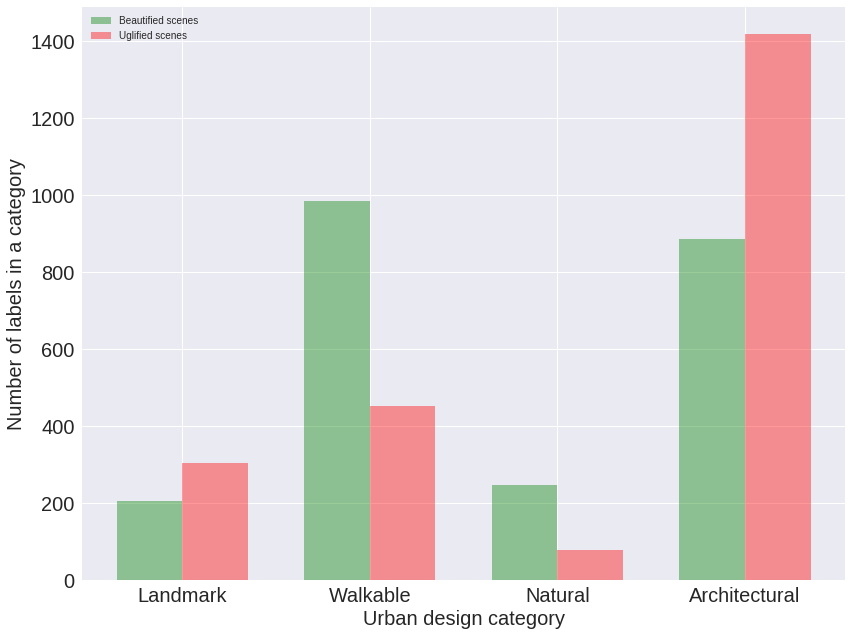
\includegraphics[width=\columnwidth]{Plot/taxonomyCount.png}
	\caption{Number of labels in specific urban design categories (on the $x$-axis) found in beautified scenes as opposed to those found in uglified scenes.}
	\label{fig:taxonomyCount}
\end{figure}


\begin{figure}[h]
	\centering
	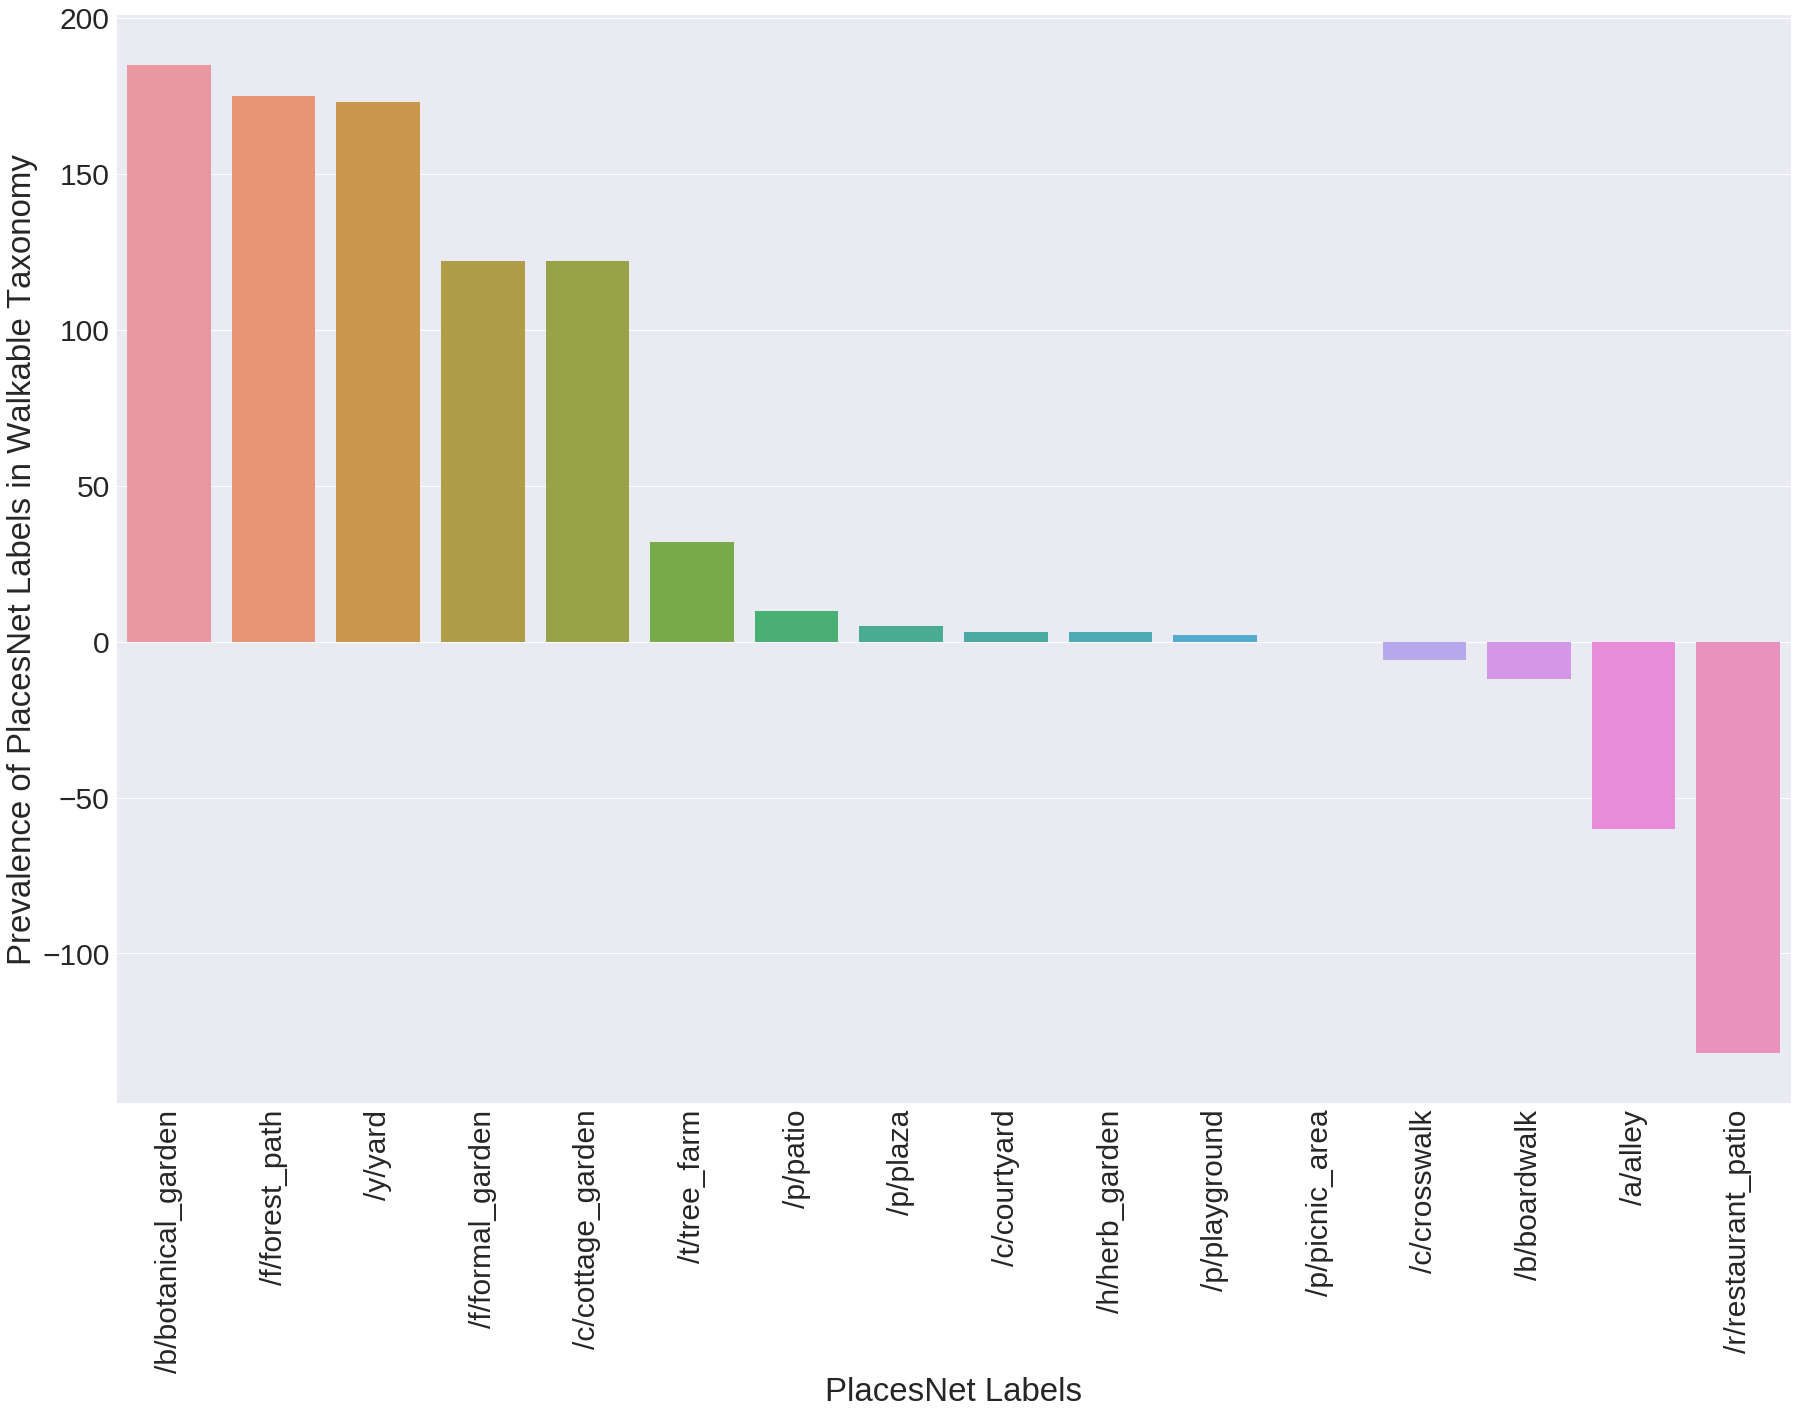
\includegraphics[width=\columnwidth]{Plot/walkable_taxonomy.png}
	\caption{Count of specific walkability-related labels  (on the $x$-axis) found in beautified scenes minus the count of the same labels found in uglified scenes.}
	\label{fig:WalkableTnomy}
\end{figure}


Having these two ways of labeling scenes, we can now test whether the expectations set by the literature of what makes urban spaces great  (Table~\ref{tab:Design_metrics}) are  met in the FaceLifted scenes. 


%**************************************************
\mbox{ } \\
\noindent
\emph{H1 Beautified scenes tend to be walkable.}
We manually select only the PlacesNet labels that are related to walkability. These labels include, for example, \textit{abbey, plaza, courtyard, garden, picnic area, \textrm{and} park}. To test hypothesis \emph{H1}, we count the number of walkability-related labels found in beautified scenes as opposed to those found in uglified scenes (Figure~\ref{fig:taxonomyCount}): the former contain twice as many walkability labels than the latter. We then determine which types of scenes are associated with beauty (Figure~\ref{fig:WalkableTnomy}). \la{Unsurprisingly, beautified scenes tend to show gardens, yards, and small paths. By contrast, uglified ones tend to show built environment features such as shop fronts and broad roads. It is worth noting that walkability often acts as an enabler for other desirable properties of places (e.g., their restorative capability). The reason why our walkability measure correlates with beauty might be because walkability acts as a proxy for such higher-order properties.}


\mbox{ } \\
%**************************************************
\noindent
\emph{H2 Beautified scenes tend to offer green spaces.}
We manually select only the PlacesNet labels that are related to greenery. These labels include, for example, \textit{fields, pasture, forest, ocean, and beach}. Then, in our 1,000 scenes, to test hypothesis \emph{H2}, we count the number of nature-related labels found in beautified scenes as opposed to those found in uglified scenes (Figure~\ref{fig:taxonomyCount}): the former contain more than twice as many nature-related labels than the latter.  To test this hypothesis further, we compute the fraction of `tree' pixels (using SegNet's label `tree') in beautified and uglified scenes, and  find that beautification adds  32\% of tree pixels, while uglification removes 17\% of them. 


\begin{figure*}[!t]
	\centering
	\hspace*{-5mm}
	\subfloat[]{
		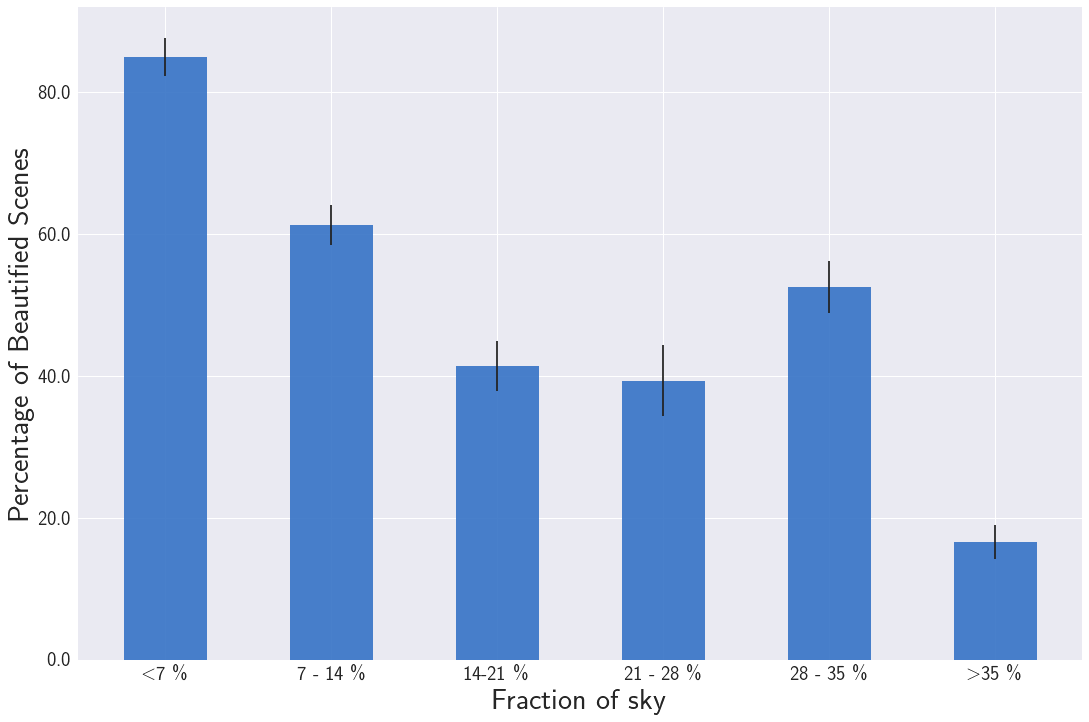
\includegraphics[width=0.45\textwidth, height = 5cm ]{Plot/BinnedPlot.png}
		\label{fig:skyBinned}
	}
	\subfloat[]{
		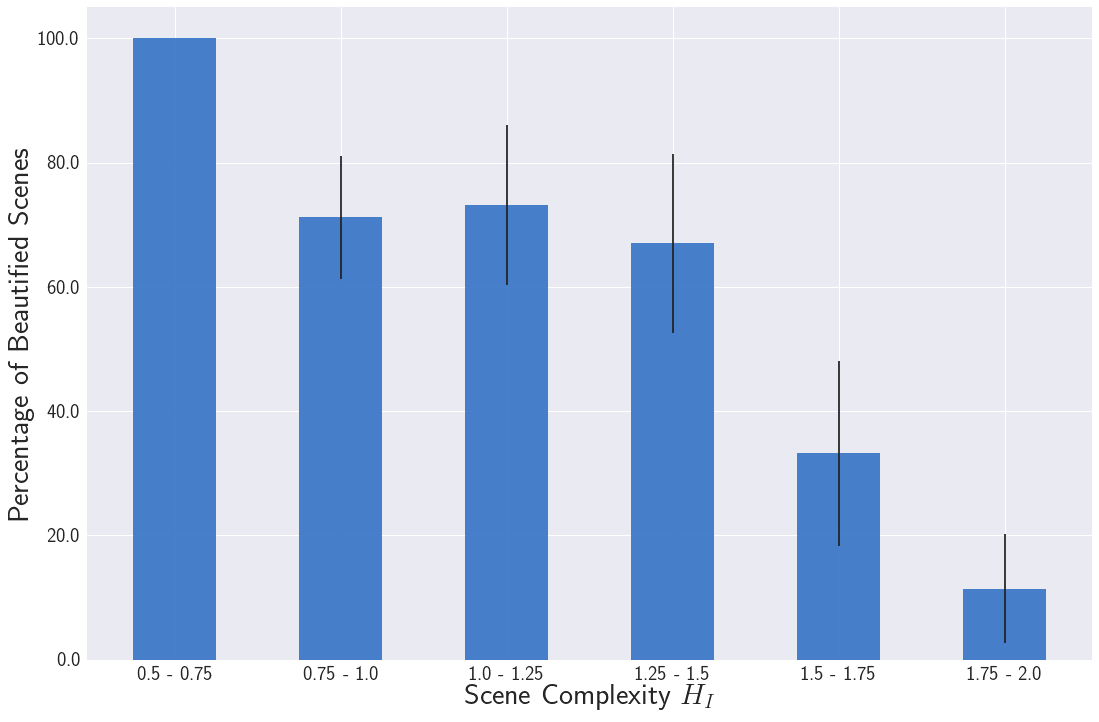
\includegraphics[width=0.45\linewidth, height = 5cm ]{Plot/binnedPlot_complexity.png}
		\label{fig:complexity}
	}
\vspace{-0.4cm}
\label{fig:bin_figures}
\caption{The percentage of beautified scenes ($y$-axis): (a) having an increasing presence of sky (on the $x$-axis); and (b) having an increasing level of visual richness  (on the $x$-axis). The error bars represent standard errors obtained by random re-sampling of the data for 500 iterations. }
\vspace{-0.4cm}
\end{figure*}



\mbox{ } \\
%**************************************************
\noindent
\emph{H3 Beautified scenes tend to feel private and `cozy'.}
To  test hypothesis \emph{H3}, we count the fraction of pixels that Segnet labeled  as `sky' and show the results in a bin plot in Figure~\ref{fig:skyBinned}:  the $x$-axis has six bins (each of which represents a given range of sky fraction), and the $y$-axis shows the percentage of beautified \emph{vs.} uglified scenes that fall into each bin.  Beautified scenes tend to be cozier (lower sky presence) than the corresponding original scenes.


\mbox{ } \\
%**************************************************
\noindent
\emph{H4 Beautified scenes tend to be visually rich.}
To quantify to which extent scenes are visually rich, we measure their visual complexity~\cite{ewing2013measuring} as  the amount of disorder in terms of distribution of (Segnet) urban elements in the scene: 
\begin{equation}
H_I = -\sum p(i)\log p(i)
\label{eq:entropy} 
\end{equation}
where $i$ is the $i^{th}$ Segnet's label, and $p(i)$ is the proportion of urban scene $I$ containing
the $i^{th}$ element. The total number of labels is twelve. The higher $H_I$, the  higher the scene's entropy, that is, the higher the scene's complexity. It has been suggested that the relationship between complexity and  pleasantness follows an `inverted U' shape~\cite{ulrich1983aesthetic}: we prefer places of medium complexity rather than places of low or high complexity. To test that, we show the percentage of beautified scenes that fall into each complexity bin  (Figure~\ref{fig:complexity}):  we do not find a strong evidence of the `inverted U' shape hypothesis, in that, beautified scenes are of low to medium complexity, while uglified ones are of high complexity.



%**************************************************
\subsection*{Q3 Urban elements characterizing beautified scenes}

\begin{table}[t!]
	\centering
	\resizebox{\linewidth}{!}{%
	\begin{tabular}{|c|c|c|c|c|}
		\hline
		\textbf{Pair of urban elements} & \textbf{$\beta_1$}  & \textbf{$\beta_2$} & \textbf{$\beta_3$}  & Error Rate (Percentage)\\
		\hline
        \hline
		Buildings - Trees & -0.032 & 0.084  & 0.005  & 12.7 \\
		\hline
		Sky - Buildings & -0.08 & -0.11 & 0.064 & 14.4 \\
		\hline
		Roads - Vehicles  & -0.015  & -0.05 & 0.023  & 40.6 \\
		\hline
		Sky - Trees & 0.03 & 0.11 & -0.012 & 12.8  \\
		\hline
		Roads - Trees & 0.04  & 0.10 &  -0.031  & 13.5  \\
		\hline
		Roads - Buildings & -0.05  & -0.097  &  0.04  & 20.2  \\
		\hline
	\end{tabular}
	}
	\caption{Coefficients of logistic regressions run on one pair of predictors at the time.}
	\label{tab:regressioncoef}
    \vspace{-10mm}
\end{table}


To determine which urban elements are the best predictors of urban beauty and the extent to which they are so, we run a logistic regression, and, to ease interpretation, we do so on one pair of predictors at the time: 
\begin{equation}
Pr(\textrm{beautiful}) = logit^{-1}(\alpha + \beta_1 * V_1 + \beta_2 * V_2  + \beta_3 * V_{1}.V_{2} )
\label{eq:regression} 
\end{equation}
where $V1$ is the fraction of the scene's pixels marked with one Segnet's label, say, ``buildings'' (over the total number of pixels),  and $V2$ is the fraction of the scene's pixels marked with another label, say, ``trees''. The result consists of three beta coefficients: $\beta_1$ reflects $V1$'s contribution in predicting beauty,  $\beta_2$ reflects $V2$'s contribution, and $\beta_3$ is the interaction effect, that is, it reflects the contribution of the dependency between $V1$ and $V2$ in predicting beauty. We run logistic regressions on the five factors that have been found to be most predictive of urban beauty~\cite{quercia2014aesthetic, ewing2013measuring, alexander1977pattern}, and show the results in Table~\ref{tab:regressioncoef}.


Since we are using logistic regressions, the quantitative interpretation of the beta coefficients is eased by the ``divide by 4 rule''~\cite{vaughn2008data}: we can take the $\beta$ coefficients and ``divide them by 4 to get an upper bound of the predictive difference corresponding to a unit difference'' in beauty~\cite{vaughn2008data}. For example, take the results in the first row of Table~\ref{tab:regressioncoef}. In the model $Pr(beautiful) = logit^{-1}(\alpha - 0.032 \cdot buildings + 0.084 \cdot trees + 0.005 \cdot  buildings \cdot trees)$, we can divide - 0.032/4 to get -0.008: a difference of 1\% in the fraction of pixels being buildings corresponds to no more than a 0.8\% \emph{negative} difference in the probability of the scene being beautiful. In a similar way, a difference of 1\% in the fraction of pixels being trees corresponds to no more than a 0.021\% \emph{positive} difference in the probability of the scene being beautiful. By considering the remaining results in Table~\ref{tab:regressioncoef}, we find that, across all pairwise comparisons, trees is the most positive element associated with beauty, while roads and buildings are the most negative ones. \la{These results match previous literature in urban design of what makes spaces great~\cite{lynch1960image,alexander1977pattern, jacobs1961death, quercia15thedigital, quercia2014aesthetic}}, adding further external validity to our framework's beautification. 




%**************************************************
\subsection*{Q4 Do architects and urban planners find it useful?}

\begin{table}[t!]
	\centering
	\resizebox{\linewidth}{!}{%
		\begin{tabular}{|c|c|c|c|c|c|}
			\hline
			\textbf{Use case} & \textbf{Definitely Not}  & \textbf{Probably Not} & \textbf{Probably}  & \textbf{Very Probably} & \textbf{Definitely}\\
			\hline
			\hline
			Decision Making & 4.8\% & 9.5\%  & 38\%  &  28.6\% & 19\%\\
			\hline
			Participatory Urban Planning & 0\% & 4.8\%  & 52.4\%  &  23.8\% & 19\%\\
			\hline
			Promote Green Cities & 4.8\% & 0\%  & 47.6\%  &  19\% & 28.6\%\\
			\hline
		\end{tabular}
	}
	\caption{Urban experts polled about the extent to which an interactive map of ``FaceLifted'' scenes promotes: (a) decision making; (b) citizen participation in urban planning; and (c) promotion of green cities}
	\label{tab:useCases}
	\vspace{-10mm}
\end{table}


%\begin{figure*}[!t]
%	\centering
%	\hspace*{-5mm}
%	\subfloat[]{
%		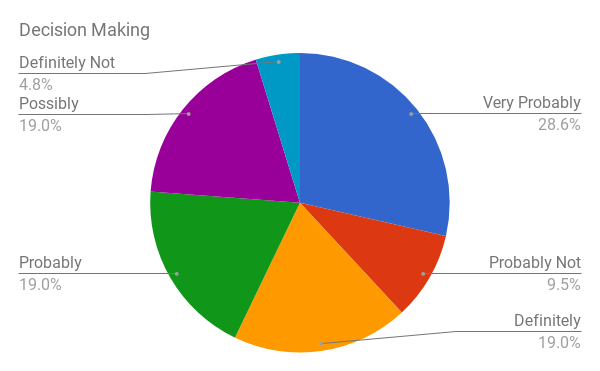
\includegraphics[width=0.3\textwidth ]{Plot/DecisionMaking.png}
%		\label{fig:decision}
%	}
%	\subfloat[]{
%		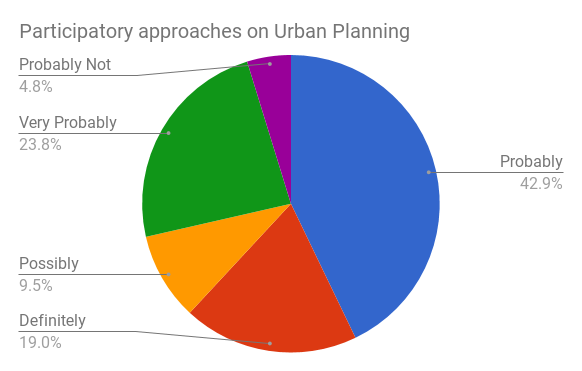
\includegraphics[width=0.3\linewidth ]{Plot/ParticipationUrbanPlanning.png}
%		\label{fig:participation}
%	}
%	\subfloat[]{
%		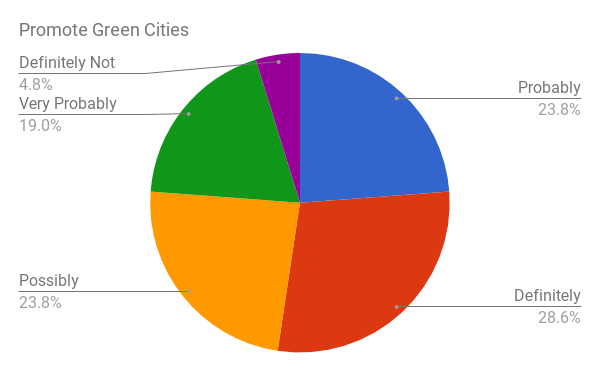
\includegraphics[width=0.3\linewidth ]{Plot/PromoteGreenCities.png}
%		\label{fig:promotion}
%	}
%%	\vspace{-0.4cm}
%	\caption{Urban experts polled about the extent to which an interactive map of ``FaceLifted'' scenes promotes: (a) decision making; (b) citizen participation in urban planning; and (c) promotion of green cities.\ns{Pie charts are not advisible. The labels are too small. You can perhaps replace this with a table.}}
%	\label{fig:pies}
%	\vspace{-0.4cm}
%\end{figure*}


\begin{figure}[t!]
	\centering
	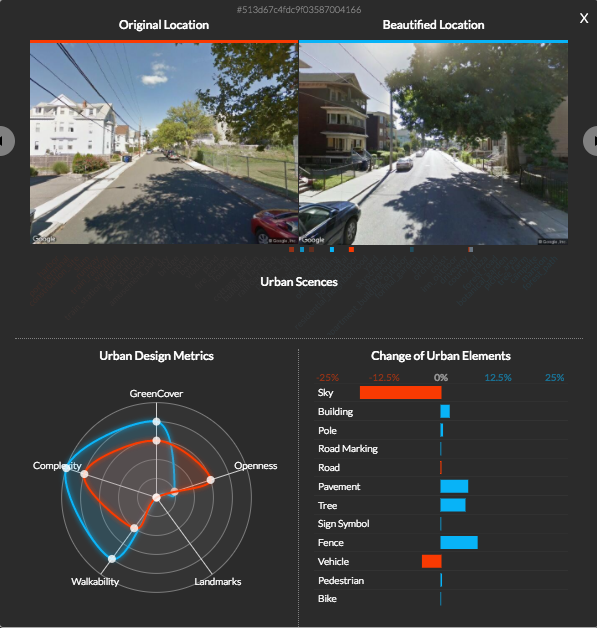
\includegraphics[width=\columnwidth]{Plot/UI.png}
	\caption{Interactive map of FaceLifted scenes in Boston.}
	\label{facelift-UI}
\end{figure}


To ascertain whether practitioners find FaceLift potentially useful, we build an interactive map of the city of Boston in which, for  selected points, we show pairs of urban scenes before/after beautification (Figure~\ref{facelift-UI}). We then send that map along with a survey to 20 experts in architecture, urban planning, and data visualization around the world. Questions were asked with a non-neutral response Likert scale (Table~\ref{tab:useCases}). That is because previous work~\cite{Agree2012,moors2008exploring} has shown that such a scale: \emph{(i)} pushes respondents to ``take a stance'', given the absence of a neutral response; and \emph{(ii)} works best if respondents are experts in the subject matter of the survey as responses of the ``I don't know'' type tend to be rare (as it is has been indeed the case for our survey). The experts had to complete tasks in which they rated FaceLift based on how well it supports decision making, participatory urbanism, and the promotion of green spaces. According to our experts (Table~\ref{tab:useCases}), the tool can very probably supports decision making, probably support participatory urbanism, and definitely promote green spaces.  These results are  also qualitatively supported by our experts' comments, which include: ``\textit{The maps reveal patterns that might not otherwise be apparent}'',  ``\textit{The tool helps focusing on parameters to identify beauty in the city while exploring it}'',  and ``\textit{The metrics are nice. It made me think more about beautiful places needing a combination of criteria, rather than a high score on one or two dimensions. It made me realize that these criteria are probably spatially correlated}''.






